\documentclass[12pt]{article}

\usepackage{times}
% \usepackage{pgfgantt}
\usepackage{amsmath, amssymb, multicol, graphicx}
% \usepackage{listing}
% \usepackage{multirow}
\usepackage{verbatim}
\usepackage{booktabs}
\usepackage{float}
\usepackage[parfill]{parskip}
\usepackage{array} \usepackage{caption}
\usepackage[colorlinks = true, linkcolor = blue]{hyperref}
\setlength{\textwidth}{6.5in}
\setlength{\textheight}{8.5in}
\setlength{\rightmargin}{0.0in}
\setlength{\leftmargin}{0.0in}
\setlength{\oddsidemargin}{0.0in}
\setlength{\parskip}{2ex}
\topmargin -0.3in 
\labelwidth = 1.2in
\labelsep = 0.1in
\parsep = 0.0in
\parindent = 0.0in
\synctex=1
\newcolumntype{+}{>{\global\let\currentrowstyle\relax}}
\newcolumntype{^}{>{\currentrowstyle}}
\newcommand{\rowstyle}[1]{\gdef\currentrowstyle{#1}%
  #1\ignorespaces }
\hfuzz=2pt
\vfuzz=2pt

\setcounter{secnumdepth}{3}
\begin{document}
\begin{titlepage}
  \centering
  Polytechnic University of Puerto Rico\\
  Hato Rey, Puerto Rico\\
  Department of Electrical and Computer Engineering and Computer
  Sciences\\
  \vspace*{15\baselineskip} \large \bfseries
  Software Requirements Specifications\\
  Smart Eyesight\\
  Version 1.0\\
  [3\baselineskip] \normalfont \vfill
  Emanuel Rivera Castro 53502\\
  Joaquin Pockels Balaguer 54012\\
  Yanilette Lopez Duprey 53990\\
  [2\baselineskip]

  \textbf{\today} \\
  COE 5002, FA-12\\
  Prof. Luis Ortiz Ortiz\\
  [2\baselineskip]
\end{titlepage}

\clearpage\pagenumbering{roman} \setcounter{page}{2}
\begin{table}[H]\centering
  \begin{tabular}{|+>{\centering\arraybackslash}m{3cm}|^>{\centering\arraybackslash}m{3cm}|^>{\centering\arraybackslash}m{3cm}|^>{\centering\arraybackslash}m{3cm}|}
    \hline
    \rowstyle{\bfseries}%
    Date & Version & Description & Author\\
    \hline
    first draft in progress & & &\\
    \hline
  \end{tabular}
  \caption[]{Revision Table}
  \label{tab:revision_table}
\end{table}
\pagebreak
\tableofcontents
\pagebreak \listoftables \pagebreak \listoffigures
\clearpage\pagenumbering{arabic}

\section{Introduction}
The present document is the Software Requirements Specifications (SRS)
for a region-based image retrieval (RBIR), feature extraction and
probabilistic neural network (PNN) classifier software application
named Smart Eyesight. The application is a salient part of a mayor
project proposal directed to the Defense Advanced Research Projects
Agency. Smart Eyesight serves as a structural model for future
extensions and provide the basic functionality for the required image
processing and classification.


\subsection{Purpose}
This Software Requirements Specifications document, establishes the
requirements, functionality, capability, behavior and design of the
software application. The document serves as a description of what the
tool should do. This SRS is to be reviewed by the project's
developers, users and client for functionality verification and
acceptance purposes.

\subsection{Intended Audience}
\label{sec:intended_audience}

This SRS is directed to:
\begin{enumerate}
\item Clients - DARPA and Prof. Arturo Geigel
\item Users - United States Armed Forces
\item Developers - AIIP/S and people responsible for maintenance and
  making updates to the system:
  \begin{itemize}
  \item Joaquin Pockels
  \item Emanuel Rivera
  \item Yanilette Lopez
  \end{itemize}
\end{enumerate}

\subsection{Project Scope}
The region-based image retrieval, features extraction and PNN
classifier tool named Smart Eyesight is mainly designed to efficiently
and effectively extract specific features from a stream of images and
classify them through a trained neural network.  Smart Eyesight is a
salient process of the DARPA's proposed system designed by Arturo
Geigel named: ``Human Computing and Machine Learning Assisted
Decentralized UAV Control''. This major system involves the
transmission of a stream of images via unmanned vehicles, a tagged
image database, a computing infrastructure to process and identify
received images, and human computer interaction between operators and
unmanned systems. Such system does not include any form of image
processing and classification, but provides the necessary objects to
do so. The large system depends on the Smart Eyesight subsystem in
order to complete the process of image identification.

The objective of the application are:
\begin{itemize}
\item Extracts relevant features from an incoming stream of images by
  using traditional features extraction algorithms and statistical
  methods
\item Train a probabilistic neural network using the relevant features
  obtained from UAV incoming images
\item Identify provided images based on its neural network training
\item Provide feedback to mayor project's interconnected inverse file
  query system.
\item Designed as an extensible software for CUDA code conversion
\item Designed as an independent system or module
\item Interconnection structure of the Smart Eyesight application with
  the main proposed system is to be established and validated with the
  consent of developers of the dependent sub-systems and the client
  himself
\end{itemize}
\cite{ImgPC}\cite{PNNSMCRFRBIR}\cite{AGMUSIUMA}\cite{RBIRSUEFD}\cite{springerlink:10.1007/s100440170015}

\subsection{Definitions and Acronyms}
This subsection shall define, or provide references to the definition
of all terms and acronyms required to properly interpret the SRS.

\subsubsection{Definitions:}
\begin{itemize}
\item \textit{Artificial Neural Network:} a neural network composed of
  interconnecting artificial neurons.
\item \textit{Artificial Neurons:} programming constructs that mimic
  the properties of biological neurons.
\item \textit{Feature Vector:} in pattern recognition and machine
  learning, it is an n-dimensional vector of numerical features that
  represent some object.
\item \textit{Independent module/system:} a fully working system which
  has no dependencies.
\item \textit{Smart Eyesight:} developed software application for
  image processing and classification.
\item \textit{Segmentation:} is the process of partitioning a digital
  image into multiple segments, with the goal of simplify and/or
  change the representation of an image into something that is more
  meaningful and easier to analyze.
\item \textit{Extensible Software:} is a software designed with future
  growth in consideration.
\item \textit{YUV:} luminance and chromiance color space used as part
  of a color image pipeline.
\end{itemize}

\subsubsection{Acronyms:}
\begin{table}[H]
  \centering
  \begin{tabular}{|+>{\lefteqn\arraybackslash}m{2cm}|^>{\lefteqn\arraybackslash}m{12cm}|}
    \hline
    \rowstyle{\bfseries}%
    Acronym & Expansion \\
    \hline
    API & Application Programming Interface \\
    \hline
    CBIR & Content Based Image Retrieval \\
    \hline
    BWF & Biorthogonal Wavelet Frame \\
    \hline
    DARPA & Defense Advanced Research Projects Agency \\
    \hline
    FRIP & Finding Region In the Pictures \\
    \hline
    GPU & Graphics Processing Unit \\
    \hline
    HDD & Hard Disk Drive \\
    \hline
    MRS & Modified Radius-based Signature \\
    \hline
    SSD & Solid-state Drive \\
    \hline
    PNN & Probabilistic Neural Network \\
    \hline
    RGB & Red Green and Blue color model\\
    \hline
    RBIR & Region Based Image Retrieval \\
    \hline
    SRS & Software Requirements Specifications \\
    \hline
    SPMP & Software Project Management Plan \\
    \hline
    TBD & To Be Described \\
    \hline
    TCP/IP & Transmission Control Protocol and Internet Protocol \\
    \hline
    UAV & Unmanned Aerial Vehicle \\
    \hline
  \end{tabular}
  \caption{Acronyms}
  \label{tab:acronyms_table}
\end{table}

\renewcommand\refname{\vskip -2cm}

\subsection{References}
\bibliographystyle{IEEEtran} \bibliography{ImageProcessingBib}

\subsection{Overview}
The rest of this document presents the full description of the RBIR
and PNN classifier tool. Section 2 is directed to the client. It shows
the general description of the application, including constrains, main
functions, user characteristics, assumptions and dependencies. Section
3 and onwards are directed to developers. They outline, in detail,
system features, specific requirements, performance, behavior,
interfaces and others.

\section{General Description}
This section presents the overall description of the application. It
explains factors that affect the application as well as its
requirements. Starting with the product perspective and ending with
assumptions and dependencies.

\subsection{Product Perspective}
Smart Eyesight serves as a multipurpose CUDA extensible software,
developed and written in C programming language that runs on a
Linux-based operating system. Smart Eyesight is an integrated
sub-system of a DARPA project proposal named: ``Human Computing and
Machine Learning Assisted Decentralized UAV Control''. It also serves
as a model structure for future mayor extensions. The system is part
of the image processing and identification infrastructure and is
resident at a Linux-based cluster as seen in the block diagram of
figure \ref{fig:SE-overall-relation}.

\begin{figure}[h]\centering
  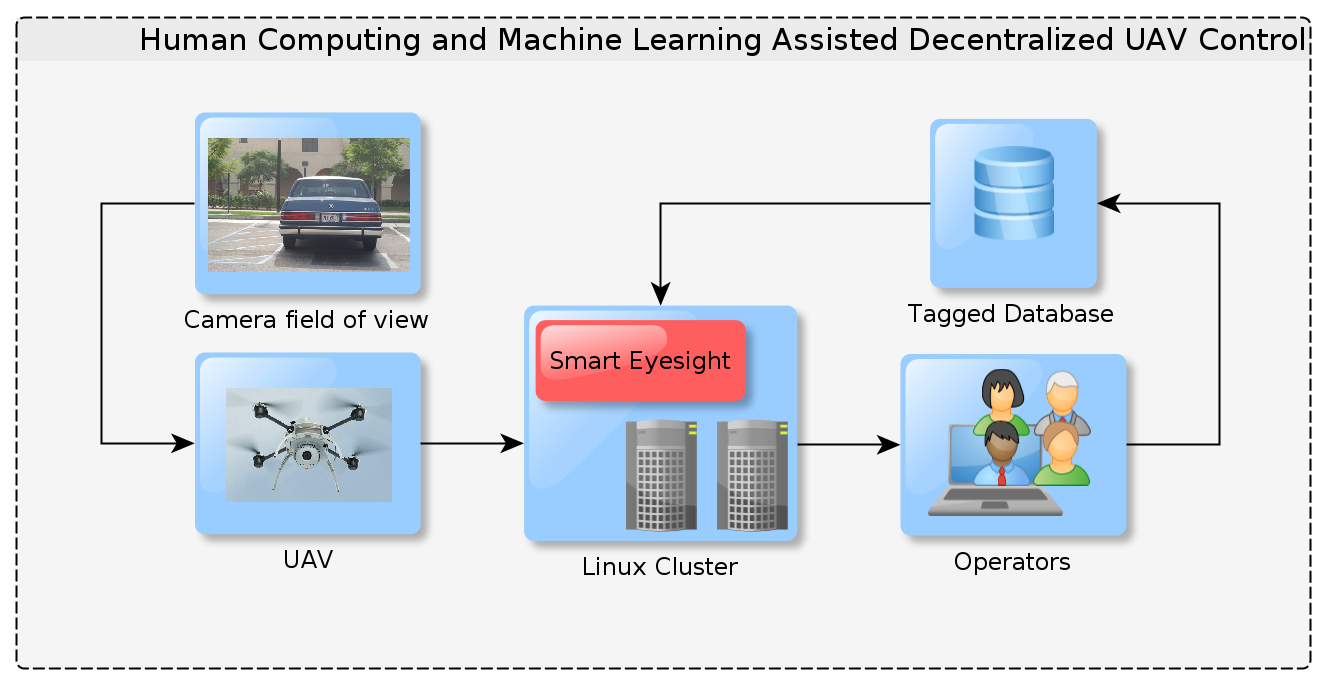
\includegraphics[width=155mm]{images/SE_relation}
  \caption{Smart Eyesight overall relation}
  \label{fig:SE-overall-relation}
\end{figure}

Essentially, the application's purpose is to identify or classify a
stream of images incoming from a tagged database and a UAV video
stream, and serve feedback to the dependant sub-systems. This is done
via two main processes and one shared process:\\

\textbf{\textit{Main processes:}}
\begin{enumerate}
\item \textbf{Neural Network Training:} this process is dedicated to
  train a probabilistic neural network using extracted features of
  regions of images from a database of tagged images.
\item \textbf{Image Classification:} this process is based on the PNN
  training, Smart Eyesight will identify each image from the extracted
  features of the UAV input stream and provide its feedback to the
  interconnected back-end sub-system.
\end{enumerate}

\textbf{\textit{Shared process:}}
\begin{enumerate}
\item \textbf{Image Processing} shared process between the Neural
  Network Training and the Image Classification tasks. This process is
  in charge of the image to segmentation and feature extraction
  conversion through a Content Based Image Retrieval process.
\end{enumerate}


\subsection{Product Functionality}
\label{sec:software_functions}
As mentioned, Smart Eyesight has two mayor processes and one
process. In this section each are briefly explained in the form of
functions. For more details refer to the section
\ref{sec:system_features}

\underline{\textbf{General Process:}} First, the probabilistic
neural network learns the characteristics of each image stored for
training purpose. These images have an identifier in the form of class
index. Both image and class gets processed in the image processing
function returning a normalized feature vector. This vector is used in
the PNN to create each image region pattern weights. Each pattern is
related to their respective class. When the external system ask for
the classification of UAV images, these images get processed the same
way by using the image processing function, thus obtaining a
normalized feature vector. Finally this vector is used in the PNN for
pattern activation and summation, leading to the selection of the
corresponding class index used by the inverse file query external
system. The whole structure is visually observable at the
communication and data flow diagram of figure
\ref{fig:function-block-diagram}.

\subsubsection{Neural Network Training}
\label{sec:NNT_function}
This function use a Probabilistic Neural Network to ``learn'' the
characteristics and properties (features) of each image by creating
and re-weighting pattern nodes per each region. It uses normalized
feature vectors produced from extracted features of image's regions
and a class per image index. The images and class index are native of
the tagged database and their conversion to feature vectors is handled
by the shared \textit{Process Image} function call. Each vector
pertain to a specific class and creates a set of connected weights
between the input layer and a new pattern in the pattern layer also
called hidden layer. These weights will latter be responsible for
``activating'' each pattern neuron in the image classification
function, thus obtaining a resultant index. The latter will be used
for the inverted file query. For more details on Probabilistic Neural
Network architecture and functionality see appendix section
\ref{sec:appendices} page \pageref{pnn_architecture}.

\begin{figure}[!h]\centering
  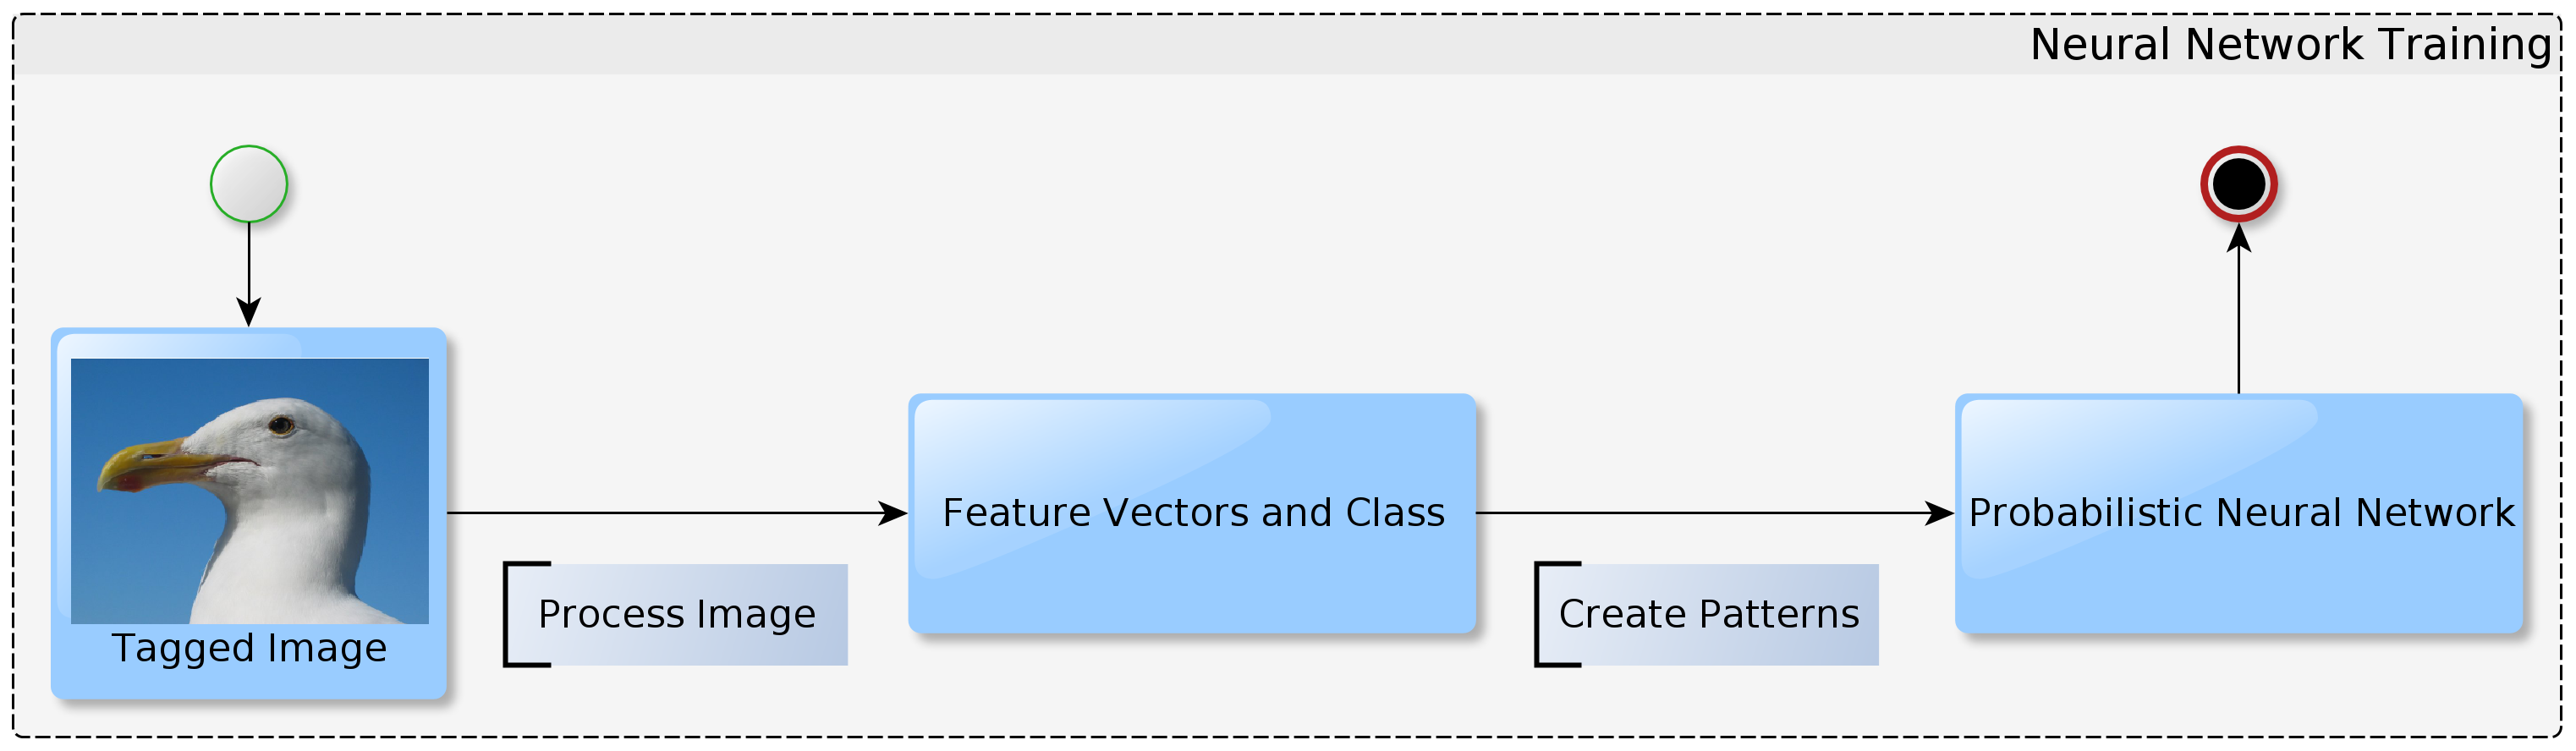
\includegraphics[width=144mm]{images/NN_training_state}
  \caption{Smart Eyesight's Neural Network Training state diagram}
  \label{fig:NN_training_state}
\end{figure}

\begin{figure}[!h]\centering
  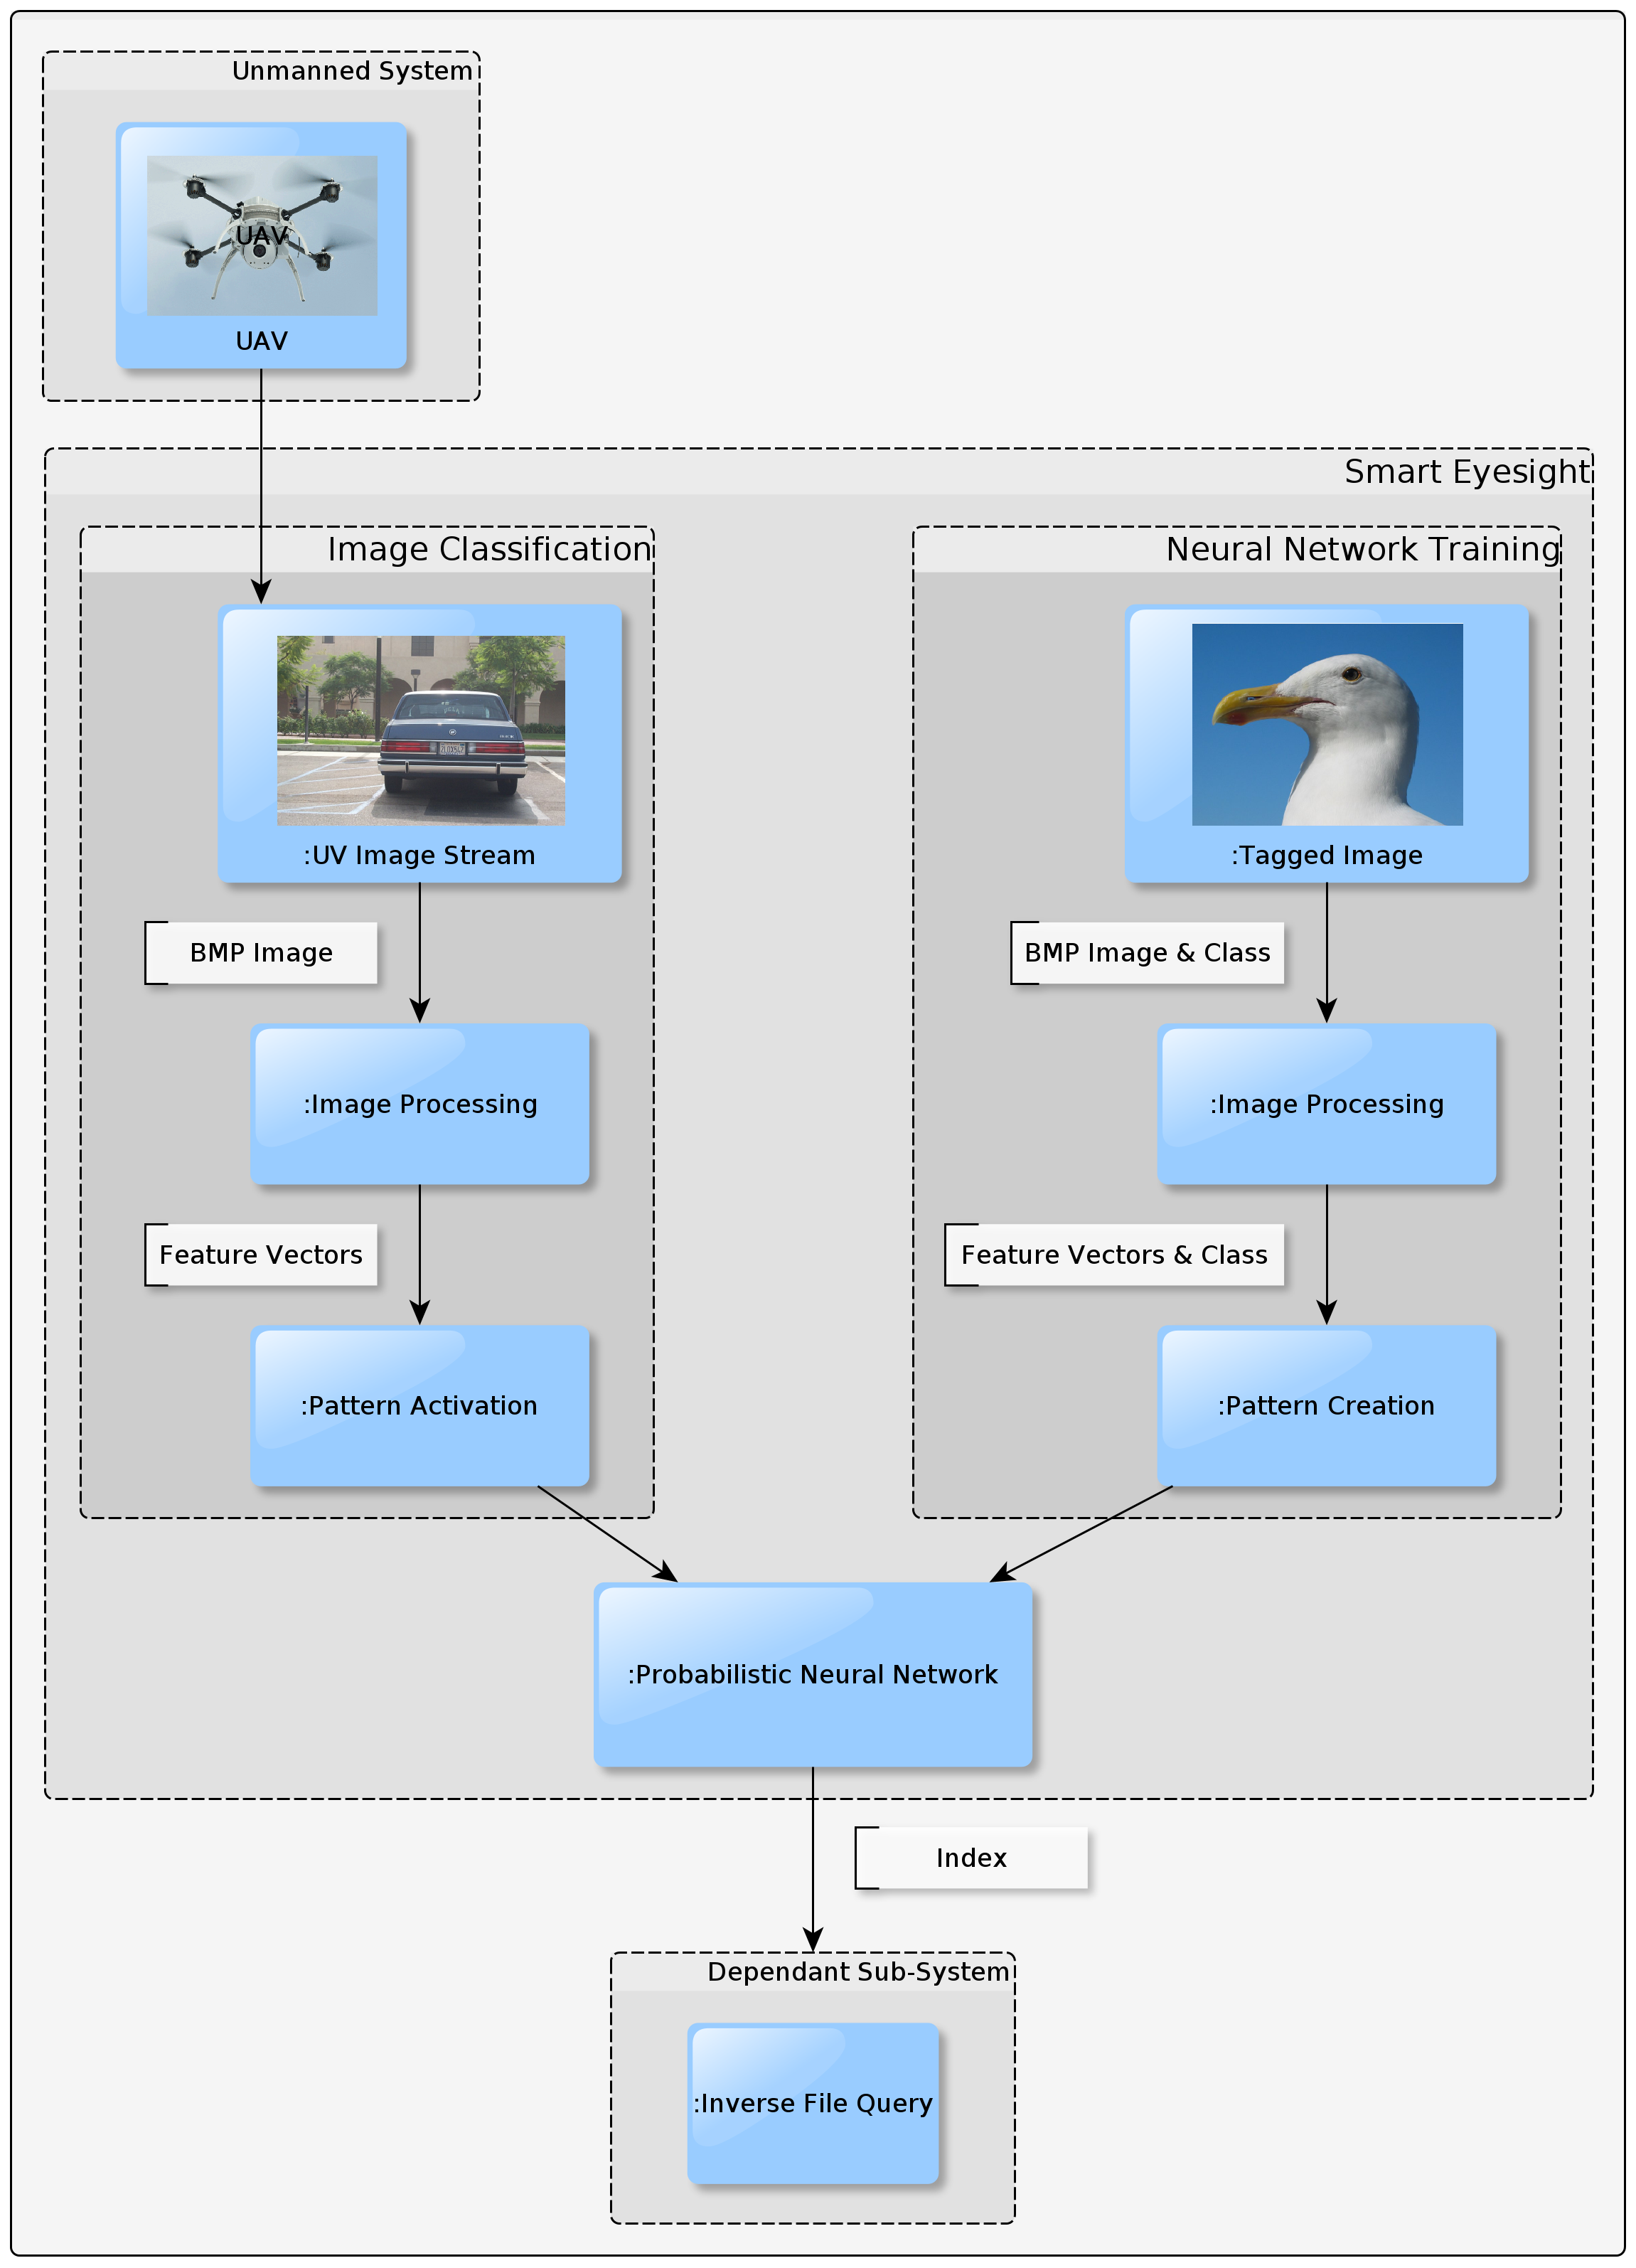
\includegraphics[width=144mm]{images/Smart_Eyesight_BD}
  \caption{Smart Eyesight communication and data flow diagram}
  \label{fig:function-block-diagram}
\end{figure}

\subsubsection{Image Classification}
\label{sec:image_classification_function}
This task use a trained Probabilistic Neural Network to ``classify''
or ``identify'' the characteristics and properties (features) of each
image by creating and re-weighting pattern nodes per each region. It
uses normalized feature vectors produced from extracted features of
image's regions. The images used for classification come from the UAV
system and their conversion to feature vectors is handled by the
shared \textit{Process Image} function call. The function uses the
feature vector to ``activate'' its pattern nodes and proceed with a
summation of their output. The result with the greatest value will
determine the class of the image in question. The function check and
compare the current feature vector with every pattern weights and
causes activation of patterns. A summation of region patter The result
of the function or final PNN layer output is an index that will be
used by the inverted file query system of the mayor system. For more
details on Probabilistic Neural Network architecture and functionality
see appendix section \ref{sec:appendices} page
\pageref{pnn_architecture}.

\begin{figure}[!h]\centering
  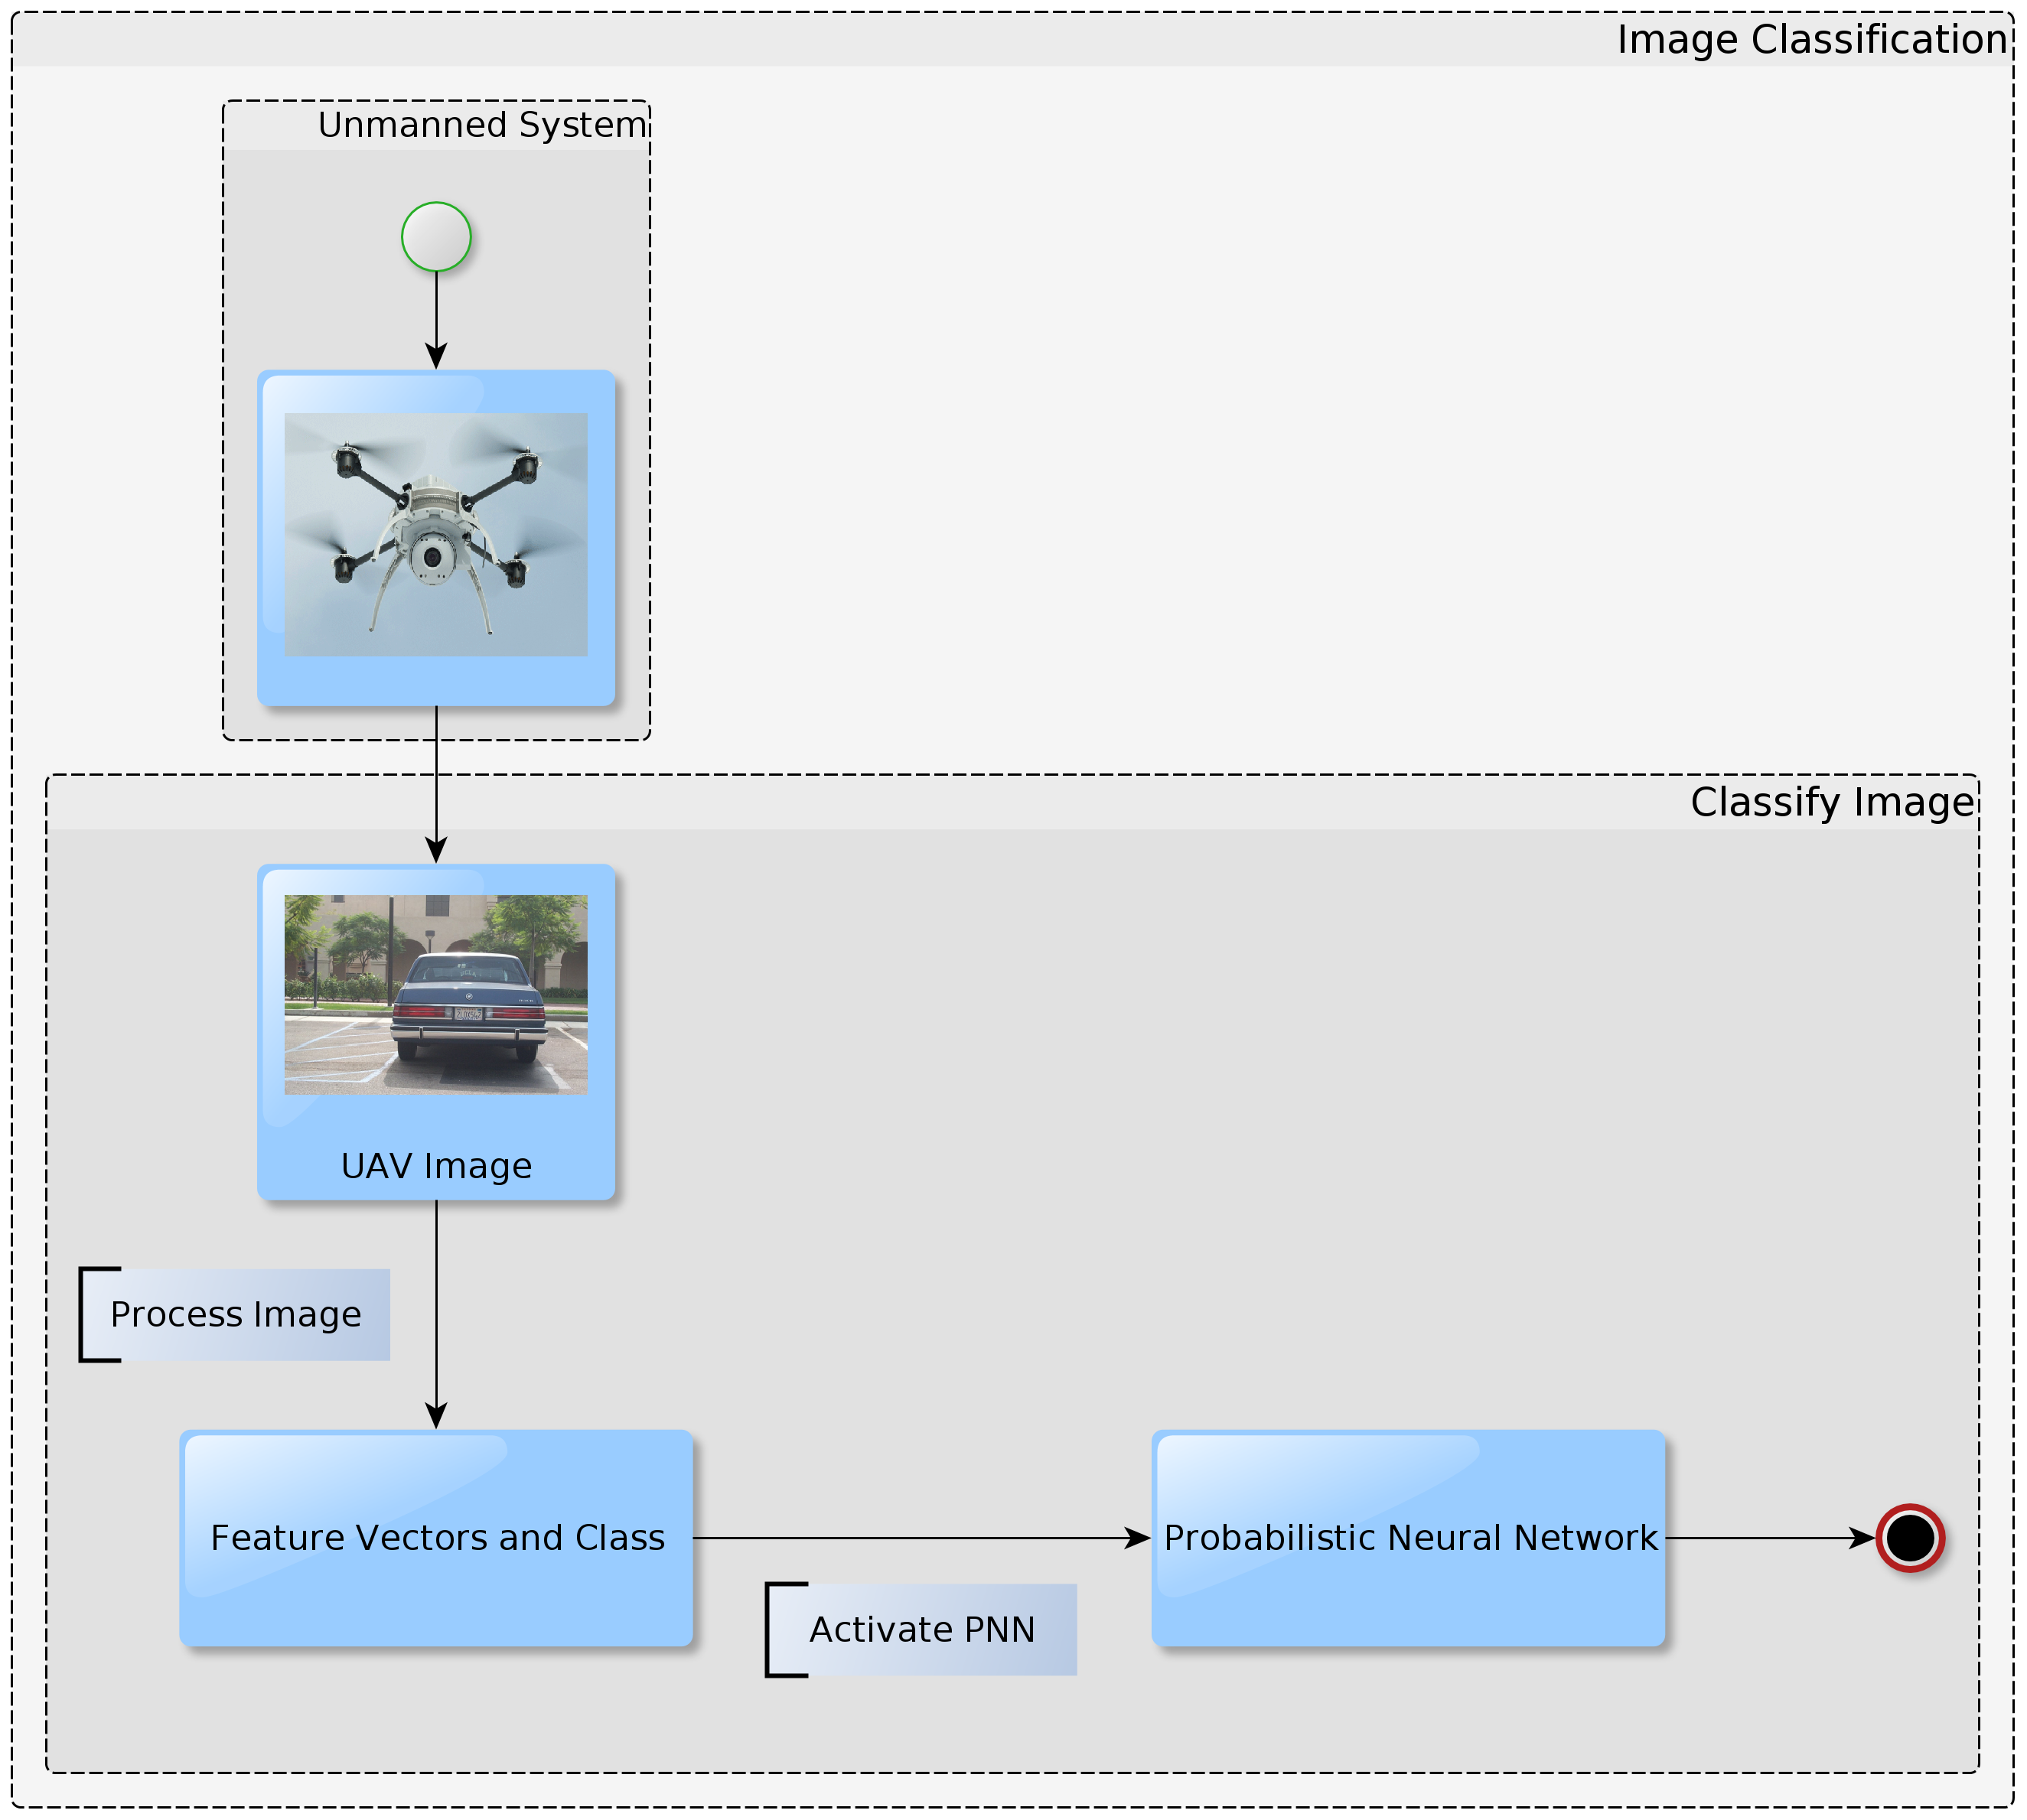
\includegraphics[width=140mm]{images/NN_classify_state}
  \caption{Smart Eyesight's Image Classification state diagram}
  \label{fig:NN_classify_state}
\end{figure}

\subsubsection{Image Processing}
\label{sec:image_processing_function}
Smart Eyesight's main Image Processing function is to describe the
content of the image by segmenting it and then extracting features of
each segmented region. That is, the semantics of image should be
extracted and stored as index. This task is possible through four
sub-functions (more details at section
\ref{sec:image_processing_feature}).

\begin{enumerate}
\item \textbf{Read Image}
\item \textbf{Segment Image}
\item \textbf{Extract Features}
\end{enumerate}

Each received image (UAV and database input) is segmented through a
retrieval system based on region called Finding Region In the Pictures
(FRIP). From each segment, five or more specific features are
extracted in order to describe effectively the image. The features to
be extracted are \textit{Color, Texture, Scale, Location and Shape}.
The extracted features are converted and normalized to a feature
vector which is used in the input layer of the PNN of both
classification and training phases. The feature vector create and
weight vectors corresponding to a class in the training face, or serve
as activation data for the testing face. Furthermore, this function
entail efficiency because of heavy use by the mentioned two processes
and vast amount of sub-functions are required to complete the task.



\subsection{Operating Environment}
The software operates in a linux-based cluster platform with resent
Ubuntu/Fedora Operating Systems. The platform is connected with the
Unmanned System through wireless access points. The training process
requires and additional cluster for continuous and efficient image
processing and training. The components of the overall system and
subsystem interconnections can be observed at figure
\ref{fig:SE-overall-relation}.

\subsection{Design and Implementation Constraints}
In this section the design and implementation constraints of the Smart
Eyesight software application are presented. Specifically and in more
detailed the image format, image processing, probabilistic neural
network and the interconnected sub-system structure.

\subsubsection{Image Constraints}
\label{sec:image_constraints}
Constraints related with the incoming images that are processed with
the FRIP method and then used in the PNN for training and
classification:
\begin{table}[H]
  \centering
  \begin{tabular}{|+>{\lefteqn\arraybackslash}m{4cm}|^>{\lefteqn\arraybackslash}m{10cm}|}
    \hline
    \rowstyle{\bfseries}%
    Object & Constraints \\
    \hline
    & BMP format \\ \cline{2-2}
    Imported Image & Header is converted to BMP format as described by the Image
    Processing in C book if necessary during image processing \\ \cline{2-2}
    & Content is converted to the RGB/YUV format if required \\ \cline{2-2}
    \hline
    Processed Images &  are stored as volatile data and are
    ``liberated'' from dynamic memory after use. \\
    \hline
  \end{tabular}
  \caption{Image Constraints Table}
  \label{tab:image_constraints}
\end{table}

\subsubsection{Image Processing Constraints}
Constraints related with the image processing functionality:
\begin{itemize}
\item Finding Regions in Picture is used as a Region Based Image
  Retrieval method
\item A circular filter, must be used to reduce noise and other
  undesirable factors of the image
\item Segmentation must be as efficient as possible
\item Extracted features should be described briefly and effectively
\item Five specific features are extracted as described in section
  \ref{sec:image_processing_function}
\item A maximum of a hundred regions are segmented per image
\end{itemize}

\subsubsection{Neural Network Constraints}
Constraints related with the Neural Network to be used for the
training and classification processes:
\begin{itemize}
\item A Probabilistic Neural Network structure is used for the
  training and classification tasks
\item For the training function, the PNN use feature vectors of
  regions of images extracted from the tagged image database
\item For the classification function, the PNN use feature vectors of
  regions of images extracted from the unmanned system's image stream
\end{itemize}

\subsubsection{Design Constraints}
Constraints related with the overall design of the whole system
including Operating System, programming language, API's and other
environments:
\begin{itemize}
\item Feedback to the interconnected dependant sub-system is in the
  form of a classification index, which format is in accordance to the
  established inverse file query structural design implemented by the
  developers in charge of the task
\item Software's code is written in C programming language
\item Linux-based Operating Systems are used to develop the
  application. Linux OS include but are not limited to Ubuntu and
  Fedora
\item Smart Eyesight software is not responsible for the application
  programming interface present between interconnected
  sub-system. Only formats will be considered as explained in this
  section.
\end{itemize}

\subsubsection{Used Tools and Technologies}
\label{sec:used_tools_and_technologies}
The following table presents specific tools and technologies that are
used in the making of Smart Eyesight:
\begin{table}[H]
  \centering
  \begin{tabular}{|+>{\lefteqn\arraybackslash}m{6cm}|^>{\lefteqn\arraybackslash}m{8cm}|}
    \hline
    \rowstyle{\bfseries}%
    Tool/Technology & Usage \\
    \hline
    C programming language & C is used as the main programming
    language. It is also used as an enabler of future extensions and
    modifications such as CUDA code conversion and parallelization. \\
    \hline
    Linux-based Operating System & Linux is used to avoid violations
    of copyrighted software's terms of use and extended costs. The
    system only uses open source shared libraries and software tools. \\
    \hline
    Book: Image Processing in C & Some libraries, designs and image processing
    code from the book are used during the development. This is an
    open source text book that contains open source code. \\
    \hline
    Personal Desktop computer and laptops & These computers are used
    for the development and design and testing of the software application and software
    engineering documents as explained in the SPMP section x. \\
    \hline
    TCP/IP and FTP & These protocols are used to obtain the UAV
    incoming images through wireless access points. Tagged incoming
    images are stored in a non-volatile device such as HDD and SSD. \\ 
    \hline
  \end{tabular}
  \caption{Used Tools and Technologies }
  \label{tab:tools_technologies}
\end{table}

\subsubsection{Regulatory Policies}
\begin{itemize}
\item At the moment, the Clients and developers have shared
  proprietary rights over Smart Eyesight. This information is
  discussed in-depth in the Smart Eyesight's SPMP document, section x.
\end{itemize}

\subsection{Assumptions and Dependencies}
Smart Eyesight has one dependency and one assumption which could
affect the requirements stated in this document. The application could
be affected if these assumptions and dependencies aren't met or
incorrect:

\begin{itemize}
\item \textbf{Dependency:} Smart Eyesight depends on the images
  incoming from the Unmanned System and tagged database.
\item \textbf{Assumption:} Images received from ether source are not
  corrupted. Meaning image headers and containing visual data have a
  fully readable header format and are considered digital images.
\end{itemize}

% \section{Specific Requirements}
% \label{sec:system_features}
% This section explains in detail each system feature and their
% respective functional and nonfunctional requirements, software and
% hardware external interfaces and other important requirements.

\section{External Interface Requirements}
This section describes the logical characteristics and communication
of each interface between the software, hardware and users.

\subsection{User Interfaces}
Not applicable

\subsection{Hardware Interfaces}
Smart Eyesight's original hardware infrastructure is composed of
Linux-based head nodes. Through the use of switches, these nodes are
connected to access points, relay servers and image processing
dedicated clusters which compose to the full system. However, since
the application serves as a model of the CUDA extended infrastructure,
most of the process is carried in a single linux OS computer and tasks
such as the PNN training in a separated cluster for a reasonable task
resolution time. Smart Eyesight obtain each UAV incoming image through
wireless connections between access points. No further hardware
requirements are needed besides the mentioned hardware constraints
mentioned in the section \ref{sec:used_tools_and_technologies}.

\subsection{Software Interfaces}
Smart Eyesight runs on recent linux-based operating systems such as
Ubuntu 1x.xx and Fedora. Dependencies are obtained through wireless
and wired TPC/IP and FTP. The software is extensible through the use
of C programming and variants such as CUDA C. The index obtained from
the classification phase is send to the dependent subsystem which uses
this information for the inverse file query task.

\subsection{Communications Interfaces}
A custom TCP/IP with FTP program is used for obtaining the
dependencies. The image processing function uses these dependencies to
create and obtain the normalized feature vectors used in the next two
phases. The training process receive feature vectors obtained from the
tagged image database. The Classification process receive feature
vectors obtained from the UAV image stream.

\section{System Features}
\label{sec:system_features}
This section list the functional requirements for Smart Eyesight by
system features.
\subsection{IP-REQ-0 Process Image}
\label{sec:image_processing_feature}

\subsubsection{Description}
This function is responsible for the efficient and effective retrieval
and description of the content of the image by using the Finding
Regions in Pictures method. As mentioned in section
\ref{sec:image_processing_function} the image processing function is
divided into four sub-function:
\begin{enumerate}
\item \textbf{Read Image}
\item \textbf{Segment Image}
\item \textbf{Extract Features}
\end{enumerate}

\subsubsection{Stimulus/Response Sequence}
The \textit{Process Image} function is called by the \textit{Neural
  Network Function} and \textit{Image Classification} functions. Each
provide an image to be processed. The data flow of the function is as
follow:

\textbf{Basic Data Flow:}
\begin{enumerate}
\item \textit{Process Image} function is called by Neural Network
  Training or Image Classification function
\item An Image file is provided by the calling function
\item \textit{Read image} function reads the image header, validates
  it and extracts necessary values such as image height and width
\item \textit{Segment Image} function segments the provided image
  through the FRIP method and stores the result in volatile memory by
  using the image header data previously obtained
\item \textit{Extract Features} function extracts all features from
  the newly created segmented image and creates a normalized feature
  vector that can be used in the PNN
\item The feature vector is returned to the calling function
\end{enumerate}

\textbf{Alternative Data Flow:} Not applicable

\subsubsection{Read Image Function}
\label{sec:read_image_function}
This process will read, validate and store the information located at
the header of the image. As mentioned in section
\ref{sec:image_constraints}, images are of BMP format. The format of
the image is described by it's file header. This format's specific
file header is simplistic. Important header fields such as file size,
image width, image height, horizontal and vertical resolutions, colors
and others are stored in memory for in order to segment the
image. Information such as image width and image height are used for
the segmentation filters as functional parameters. The matrix of
pixels information is stored in memory together with the obtained
header information in order to be used by the next task (image
segmentation). For more details of the BMP image format refer to the
appendix section \ref{sec:appendices} page \pageref{bmp_header}.

\subsubsection{Segment Image Function}
\label{sec:segment_image_function}
In this process, image segmentation refers to partitioning an image
into different regions that are homogeneous or similar in image
characteristics. To do this new space is opened in dynamic memory to
store the segmented image by using the extracted header information
obtained form the \textit{Read Image} sub-function. The segmentation
function use traditional algorithms and statistical methods to segment
each frame. In this case we use Finding Regions in Picture, which
segments an image into regions using scaled and shifted color, CIE
L*a*b* color and edge distribution of image.

In details, the FRIP process include the use of an adaptive circular
filter, which coarsely quantize the image's color, and a region
iterative merging and labeling. As an extension to this system the
segmentation will be parallelized and clustered for optimization
purposes. In figure \ref{fig:segmented_images} we can observe an
example of segmented images by using FRIP.
\begin{figure}[!h]\centering
  \includegraphics[width=100mm]{images/Untitled}
  \caption{Segmented images example}
  \label{fig:segmented_images}
\end{figure}

\textbf{\underline{Finding Region in Picture (FRIP) process}}

\begin{enumerate}
\item \textit{Adaptive Circular Filter:} CIE L*a*b* and RGB color
  space is used to represent color features. CIE L*a*b* color space is
  generated by linearly transforming the RGB color space to the XYZ
  color space by a nonlinear transformation. After the transformation,
  images are smoothed to remove noise using a median filter. Then the
  adaptive (7x7, 11x11, 15x15 pixels) circular filter is applied.
\item \textit{Iterative Level Using Region Labeling and Iterative
    Region Merging:} After the first-level segmentation, some regions
  may be declared to be similar if they have similar color properties,
  even though they are in fact semantically different
  regions. Therefore, each region is labeled as different regions
  using the connected-component algorithm. In the step, different
  region numbers are assigned to each region.

  After region labeling, if the number of regions is over 30, we
  repeat the circular filtering starting with the smallest filter
  (7x7) in order to merge small patches into adjacent regions that are
  not merged at the first level, and then perform region merging with
  a modifiable threshold T. We restrict the maximum number of regions
  to TBD.
\end{enumerate}

The whole process is observable at figure \ref{filter_process}

\begin{figure}[!h]
  \centering
  \includegraphics[width=100mm]{images/Adaptive_circular_filter}
  \caption{Image segmentation using adaptive circular filter and
    region labeling/merging}
  \label{filter_process}
\end{figure}

\subsubsection{Extract Features Function}
\label{sec:extract_features_function}
From the segmented image, features are extracted from each
region. Features extracted from each region are normalized and
converted to a feature vector. We extract five specific features from
each regions:
\begin{table}[H]
  \centering
  \begin{tabular}{|+>{\lefteqn\arraybackslash}m{3cm}|^>{\lefteqn\arraybackslash}m{11cm}|}
    \hline
    \rowstyle{\bfseries}%
    Feature & Details \\
    \hline
    Color & The average color of RGB(Ar, Ag, Ab) and CIE
    L*a*b*(Al, Aa, Ab) color space \\
    \hline
    Texture & The Biorthogonal Wavelet Frame(BWF) \\
    \hline
    Scale/NArea & Size of the region in NArea form. That is number
    of pixels of a region divided by the image size \\
    \hline
    Location & Centroid of the region \\
    \hline
    Shape & Eccentricity and Modified Radius-based Signature \\
    \hline
  \end{tabular}
  \caption{Region specific extracted features}
  \label{tab:region_specific_extracted_features}
\end{table}

All extracted features are then normalized to 0 - 1. Afterwards all
features from a region are converted to a feature vector for latter
PNN use. This function concludes the \textit{Image Processing}
presented feature.

\subsubsection{Functional Requirements}
\begin{itemize}
\item IP-REQ-1: Image segmentation Region-Based Image Retrieval
  application shall be the Finding Regions in Picture
\item IP-REQ-2: Five specific features found at table
  \ref{tab:region_specific_extracted_features} shall be extracted
  from the segmented image's regions
\item IP-REQ-3: Maximum number of regions shall be 100
\end{itemize}

\subsection{T-REQ-0 Train PNN}
\label{sec:nn_training_feature}
\subsubsection{Description}

The requirements for this task are as follow:
\begin{itemize}
\item T-REQ-1: Use a Probabilistic Neural Network for training
\item T-REQ-2: The PNN use normalized feature vectors as input
\item T-REQ-3: The feature vectors used in the PNN are extracted from the
  \textit{image processing} shared process
\item T-REQ-4: Images and class per image index used in this function are
  provided by the tagged image database
\end{itemize}
\subsection{C-REQ-0 Classify Image}
\label{sec:image_classification_feature}
\subsubsection{Description}

The requirements for this task are as follow:
\begin{itemize}
\item C-REQ-1: Use a Probabilistic Neural Network for classifying images
\item C-REQ-2: The PNN use normalized feature vectors as input
\item C-REQ-3: The feature vectors used in the PNN are extracted from the
  \textit{Image Processing} shared process
\item C-REQ-4: Images used in this function are provided by the UAV
\end{itemize}


\section{Other Nonfunctional Requirements}
\label{sec:nonfunctional_requirements}
\subsection{Performance Requirements}
\subsection{Software Quality Attributes}
\subsection{Other Requirements}
\subsection{Appendices}
\label{sec:appendices}
\begin{figure}[h]\centering
  \includegraphics[width=150mm]{images/PNN_Architecture}
  \caption{PNN architecture}
  \label{pnn_architecture}
\end{figure}
\begin{figure}[h]\centering
  \includegraphics[width=40mm]{images/BMP_header}
  \caption{BMP header architecture}
  \label{bmp_header}
\end{figure}
\begin{figure}[h]\centering
  \includegraphics[width=50mm]{images/BMP_header_bitmap}
  \caption{BMP header BitMap architecture}
  \label{bmp_header_bitmap}
\end{figure}
\end{document}